\documentclass[aps, 12pt]{revtex4}
\usepackage[english]{babel}
\usepackage[utf8]{inputenc}
\usepackage[T1]{fontenc}
% \usepackage{NotesTeX}
\usepackage{subfigure}
\usepackage{tikz}
\usetikzlibrary{arrows}
\usepackage{multirow}
\usepackage{listings}
\usepackage{extarrows}
\usepackage{parskip}
\usepackage{eurosym}
\usepackage{footmisc}
\usepackage{kantlipsum}
\usepackage{algorithm}
\usepackage{algpseudocode}


\def\thesection{\arabic{section}}

\renewcommand{\deg}{^{\circ}}
\newcommand\numberthis{\addtocounter{equation}{1}\tag{\theequation}}
\newcommand{\hksqrt}[2][]{\ \mathpalette\DHLhksqrt{[#1]{#2\,}}}
\def\DHLhksqrt#1#2{\setbox0=\hbox{$#1\sqrt#2$}\dimen0=\ht0
    \advance\dimen0-0.3\ht0
    \setbox2=\hbox{\vrule height\ht0 depth -\dimen0}
    {\box0\lower0.65pt\box2}}

\graphicspath{{figs/}}
\newcommand{\includegraphicsmaybe}[2][]{\IfFileExists{../plots/#2}{\includegraphics[#1]{#2}}{\includegraphics[width=0.7\linewidth]{giffel.jpg}}}



\begin{document}

\author{Håkon Olav Torvik}
\title{\Huge Problem Set 2 \\ \small Math228B Numerical solutions to differential equations}
\affiliation{UC Berkeley}
\date{\today}


\maketitle

\section*{Problem 1}
\subsection*{Part a, See previous problem set}

\subsection*{Part b}
We have the method
\begin{equation}\label{eq:method}
    U_j^{n+1} = U_j^n + \frac{k\kappa}{2h^2}\left[U_{j-1}^n - 2U_j^n + U_{j+1}^n + U_{j-1}^{n+1} -2U_j^{n+1}+U_{j+1}^{n+1} \right] - k\gamma \left[(1-\theta)U_j^n+\theta U_j^{n+1}\right],
\end{equation}
which models diffusion with decay.

Let
\begin{equation}\label{eq:vonneumann}
    U_j^n = e^{ijh\xi}, \hspace{3mm} U_j^{n+1} = g(\xi)U_j^n.
\end{equation}

Von Neumann analysis says that the method is stable provided $|g|\leq 1$.

Inserting \eqref{eq:vonneumann} into \eqref{eq:method}, we get the expression for $g(\xi)$ as
\begin{align*}
    ge^{ijh\xi} =                     & e^{ijh\xi} + \frac{k\kappa}{2h^2}\left[e^{i(j-1)h\xi} - 2e^{ijh\xi} + e^{i(j+1)h\xi} + ge^{i(j-1)h\xi} - 2ge^{ijh\xi} + ge^{i(j+1)h\xi} \right]
    \\
                                      & - k\gamma \left[(1-\theta)e^{ijh\xi}+\theta ge^{ijh\xi}\right],
    \\
    g =                               & 1 + \frac{k\kappa}{2h^2}\left[e^{-ih\xi}-2+e^{ih\xi} +ge^{-ih\xi} - 2g + ge^{ih\xi} \right] - k\gamma\left[(1-\theta)+\theta g\right],
    \\
    g =                               & 1 + \frac{k\kappa}{h^2}\left[\cos{(h\xi)} -1 + g\cos{(h\xi)}-g\right] + k\gamma(\theta-1)-k\gamma\theta g,
    \\
    g - \lambda g + k\gamma\theta g = & 1 + \lambda +k\gamma(\theta-1), \hspace{20mm} \text{where} \hspace{3mm} \lambda \equiv \frac{k\kappa}{h^2}\left(\cos{(h\xi)}-1\right),
    \\
    g =                               & \frac{1+\lambda +k\gamma(\theta - 1)}{1-\lambda +k\gamma\theta}.
\end{align*}

Using the stability condition $|g|\leq 1$, we get
\begin{align*}\label{eq:ineq}
    1\geq                                       & \left|\frac{1+\lambda +k\gamma(\theta - 1)}{1-\lambda +k\gamma\theta}\right|, \numberthis
    \\
    \left|1-\lambda +k\gamma\theta \right| \geq & \left|1+\lambda +k\gamma(\theta - 1)\right|.
\end{align*}
In the second step I used the fact that $\lambda$ is always negative or equal to $0$, such that $1-\lambda+k\gamma\theta > 1$. WolframAlpha gives that under the conditions $\lambda < 0$ and $k\gamma>0$, both of which are obviously always true, then
\begin{equation*}
    \theta \geq \frac{k\gamma-2}{2k\gamma} = \frac{1}{2} - \frac{1}{k\gamma}.
\end{equation*}
Again, as $k$ and $\gamma$ are both non-negative, the second term can be dropped, and the method is unconditionally stable for any
\begin{equation*}
    \theta \geq \frac{1}{2},
\end{equation*}
which is what was to be shown. (The conditions set are already true from the formulation of the problem).

\subsection*{c}
Going back to \eqref{eq:ineq}, I now set $\theta = 0$, and do a similar analysis.

\begin{align*}
    1           & \geq \left|\frac{1+\lambda -k\gamma}{1-\lambda}\right|,
    \\
    |1-\lambda| & \geq |1+\lambda -k\gamma|.
\end{align*}
Again, WolframAlpha, under the conditions that the solutions are real and $\lambda < 1$, both of which are again always true, gives the solution as $2\lambda \leq k\gamma \leq 2$. As $\lambda<0$, the first inequality is always upheld. This gives unconditional stability for $k\leq 2/\gamma$, which is what was to be shown.


\section*{Problem 2}
To solve the differential equation
\begin{equation*}
    u_t +au_x =0,
\end{equation*}
one could use the following scheme
\begin{equation*}
    U_j^{n+1} = U_{j-2}^{n-1}-\left(\frac{ak}{h}-1\right)(U_j^n-U_{j-2}^n).
\end{equation*}

\subsection*{Part a}
To determine the order of accuracy of the method, I Taylor expand, and subtract the 2 sides from eachother. I Taylor expand to 3rd order.
\begin{align*}
    U_j^n     & = u(x, t)  \equiv u
    \\
    u(x, t+k) & = u(x-2h, t-k)-\left(\frac{ak}{h}-1\right)(u(x,t)-u(x-2h,t))
\end{align*}
\begin{align*}
    u(x, t+k)     = & u +ku_t + \frac{k^2}{2}u_{tt}+\frac{k^3}{6}u_{ttt} + \mathcal{O}(k^4)
    \\
    u(x-2h, t)   =  & u-2hu_x + \frac{4h^2}{2}u_{xx} - \frac{8h^3}{6}u_{xxx} + \mathcal{O}(h^4)
    \\
    u(x-2h, t-k) =  & u - 2hu_x - ku_t + \frac{1}{2}\left[4h^2u_{xx} + 2\cdot 2hku_{xt}+k^2u_{tt} \right] +
    \\
                    & + \frac{1}{6}\left[-8h^3u_{xxx}-3\cdot4h^2ku_{xxt}-3\cdot2hk^2u_{xtt}-k^3u_{ttt} \right] + \mathcal{O}(h^4+k^4)
\end{align*}
\begin{align*}
    \tau = & u - 2hu_x - ku_t + \frac{1}{2}\left[4h^2u_{xx} + 2\cdot 2hku_{xt}+k^2u_{tt} \right] \\&+ \frac{1}{6}\left[-8h^3u_{xxx}-12h^2ku_{xxt}-6hk^2u_{xtt}-k^3u_{ttt} \right] \\ &- \left(\frac{ak}{h}-1\right)u + \left(\frac{ak}{h}-1\right)\left[u-2hu_x + \frac{4h^2}{2}u_{xx} - \frac{8h^3}{6}u_{xxx} \right] \\ & - \left(u +ku_t + \frac{k^2}{2}u_{tt}+\frac{k^3}{6}u_{ttt}\right) + \mathcal{O}(kh^3+k^4)
    \\
    =      & \frac{k}{3}\left(\frac{2h^2}{a} + ak^2 - 3hk\right)u_{xxx} + \mathcal{O}(kh^3+k^4)
    \\
    =      & \mathcal{O}(h^2k + k^3 + hk^2)
\end{align*}
where I have used the original equation $u_t=-au_x$ to cancel all frist-derivatives and second-derivatives of $u$, as well as many of the thrid-derivatives using the following relations.
\begin{align*}
    u_t                                       & = -au_x
    \\
    u_{tt} = -au_{xt} \hspace{2mm}            & \hspace{2mm} u_{tx}   = -au_{xx}
    \\
    u_{ttt}  = -au_{xtt} \hspace{4mm} u_{ttx} & = -au_{xxt} \hspace{4mm} u_{txx} = -au_{xxx}
\end{align*}
This seems to be a 3rd order method.

\subsection*{Part b}
The true solution to the advection equation for a point is the value of the point upstream at the previous timestep. The skewed leapfrog method with $\nu \equiv ak/h = 1$ will depend on the point two steps back in time, and two upstream, so this is also okay. But for values near 1 it will depend on grid-point outside the true domain of dependence and thus not satisfy the CLF-condition.


\subsection*{Part c}
Again, I use the definitions \eqref{eq:vonneumann}.
\begin{align*}
    u_j^{n+1}=          & u_{j-2}^{n-1}-(\nu - 1)(u_j^n - u_{j-2}^n), \hspace{4mm} \nu \equiv ak/h
    \\
    \Downarrow          &
    \\
    ge^{i\xi hj} =      & e^{i\xi h(j-2)}/g -(\nu -1)(e^{i\xi hj} - e^{i\xi h(j-2)})
    \\
    g =                 & e^{-2i\xi h} / g - \nu + \nu e^{-2i\xi h}
    + 1 - e^{-2i\xi h}
    \\
    \gamma ^2 =         & 1 - \nu\gamma e^{i\xi hj} + \nu g + \gamma e^{i\xi h}-g, \hspace{4mm} \gamma \equiv ge^{i\xi h}
    \\
    g\gamma^2 =         & g - \nu\gamma^2 + \nu g^2 + \gamma^2-g^2
    \\
    \gamma^2(g+\nu-1) = & g(1+\nu g - g)
    \\
    \gamma^2 =          & g\frac{(1+\nu g - g)}{(g+\nu-1)}
\end{align*}
For $|g| = |\gamma| \geq 1$, I get that $\nu=0 \land \nu=1 \land |\nu| \geq 2 $ will satisfy the sability condition. This was found by plotting $\gamma^2(\nu)$ for $|g|\geq 1$ and finding the regions where it was always less than 1.

This is similar to what I found in the previous part, but with the addition of courant numbers larger than $2$.


\section*{Problem 3}
\subsection*{Part a-e}
Code, implemented in the Julia-code uploaded on bCourses. The functions I implemented for part b, c, d and e have different signatures than what was specified in the problem set. I therefore also added some wrapper-functions with the specified signature so autograder would be happy. I have not tested these, but they are very small, so should work alright.

\subsection*{Part f}
I implement a solver that sets up the system and iterates to the final solution. I use the max-norm to find the error from the exact solution among all solution components. Figure \ref{fig:convergence} shows a log-log plot of the error against the step length $h$ for the 2 specified filter-parameters $\alpha$. For $\alpha=0.499$ I get that the slope is $4.257$, while for $\alpha=0.480$, it is $2.971$.

$\alpha=0.5$ corresponds to no filtering, so I get better results using less filtering for smaller step sizes. This is as expected, as filtering is not a correct operation when solving such differential equations, but is in this case needed to avoid the solution blowing up. Therefore, as I get a bigger grid, less filtering will be closer to the true solution, while for smaller grids, I need to filter more to maintain stability.

\begin{figure}
    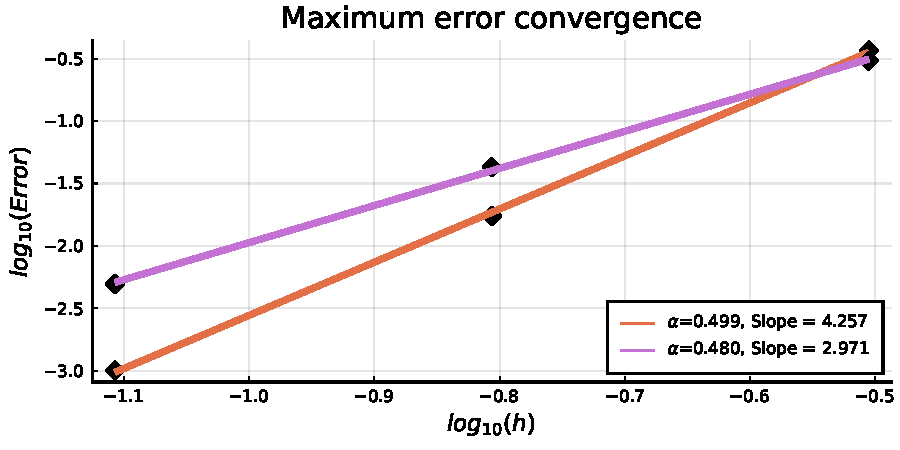
\includegraphics[width=\linewidth]{vortex_convergence.pdf}
    \caption{Convergence-plot of the error as the spatial step length gets smaller, for 2 different values of the filtering-parameter $\alpha$.}
    \label{fig:convergence}
\end{figure}

\subsection*{Part g}
I implement the specified intital conditions and use my RK4-solver. At $T=1$, I plot the density of the system in the domain, which is shown in Figure \ref{fig:KelvinHelmholtz}. The results looks reasonable.

\begin{figure}
    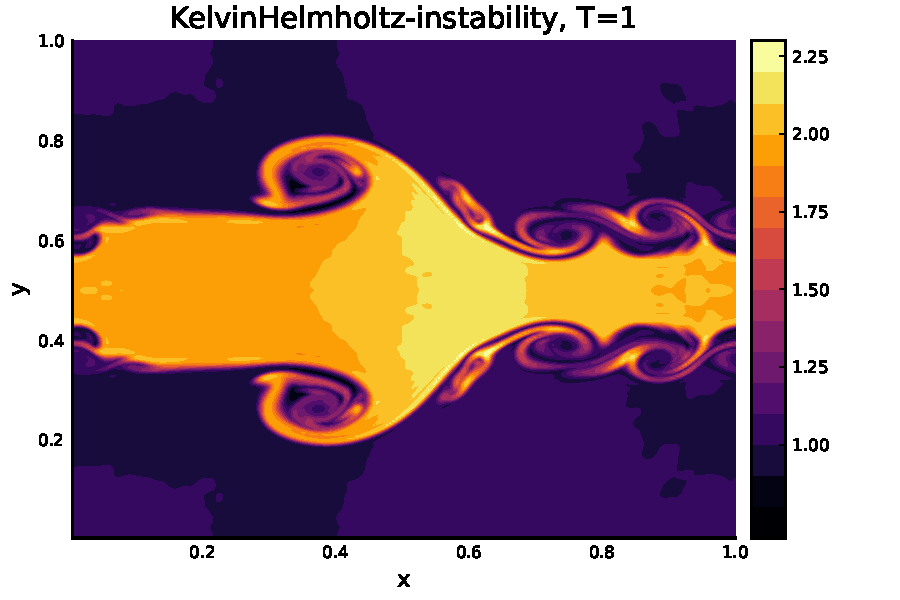
\includegraphics[width=\linewidth]{KelvinHelmholtz.pdf}
    \caption{The simulated Kelvin-Helmholtz instability at $T=1$.}
    \label{fig:KelvinHelmholtz}
\end{figure}




\begin{thebibliography}{99}
\end{thebibliography}

\end{document}

